\documentclass[12pt]{report}
\usepackage[utf8]{inputenc}
\usepackage[russian]{babel}
%\usepackage[14pt]{extsizes}
\usepackage{listings}
\usepackage{graphicx}
\usepackage{amsmath,amsfonts,amssymb,amsthm,mathtools} 
\usepackage{pgfplots}
\usepackage{filecontents}
\usepackage{float}
\usepackage{comment}
\usepackage{indentfirst}
\usepackage{eucal}
\usepackage{enumitem}
%s\documentclass[openany]{book}
\frenchspacing

\usepackage{indentfirst} % Красная строка

\usetikzlibrary{datavisualization}
\usetikzlibrary{datavisualization.formats.functions}

\usepackage{amsmath}



\usepackage{listings}

\lstset{
    language=c,
    basicstyle= \footnotesize,
    breakatwhitespace=true,
    breaklines=true,
    inputencoding=utf8,
    numbers=left,
    numberstyle=\footnotesize,
    showspaces=false,
    showstringspaces=false,
    showtabs=false,
    stepnumber=1,
    tabsize=4,
    frame=single,
    escapebegin=\begin{russian}\commentfont,
    escapeend=\end{russian},
    literate={Ö}{{\"O}}1
    {Ä}{{\"A}}1
    {Ü}{{\"U}}1
    {ß}{{\ss}}1
    {ü}{{\"u}}1
    {ä}{{\"a}}1
    {ö}{{\"o}}1
    {~}{{\textasciitilde}}1
    {а}{{\selectfont\char224}}1
    {б}{{\selectfont\char225}}1
    {в}{{\selectfont\char226}}1
    {г}{{\selectfont\char227}}1
    {д}{{\selectfont\char228}}1
    {е}{{\selectfont\char229}}1
    {ё}{{\"e}}1
    {ж}{{\selectfont\char230}}1
    {з}{{\selectfont\char231}}1
    {и}{{\selectfont\char232}}1
    {й}{{\selectfont\char233}}1
    {к}{{\selectfont\char234}}1
    {л}{{\selectfont\char235}}1
    {м}{{\selectfont\char236}}1
    {н}{{\selectfont\char237}}1
    {о}{{\selectfont\char238}}1
    {п}{{\selectfont\char239}}1
    {р}{{\selectfont\char240}}1
    {с}{{\selectfont\char241}}1
    {т}{{\selectfont\char242}}1
    {у}{{\selectfont\char243}}1
    {ф}{{\selectfont\char244}}1
    {х}{{\selectfont\char245}}1
    {ц}{{\selectfont\char246}}1
    {ч}{{\selectfont\char247}}1
    {ш}{{\selectfont\char248}}1
    {щ}{{\selectfont\char249}}1
    {ъ}{{\selectfont\char250}}1
    {ы}{{\selectfont\char251}}1
    {ь}{{\selectfont\char252}}1
    {э}{{\selectfont\char253}}1
    {ю}{{\selectfont\char254}}1
    {я}{{\selectfont\char255}}1
    {А}{{\selectfont\char192}}1
    {Б}{{\selectfont\char193}}1
    {В}{{\selectfont\char194}}1
    {Г}{{\selectfont\char195}}1
    {Д}{{\selectfont\char196}}1
    {Е}{{\selectfont\char197}}1
    {Ё}{{\"E}}1
    {Ж}{{\selectfont\char198}}1
    {З}{{\selectfont\char199}}1
    {И}{{\selectfont\char200}}1
    {Й}{{\selectfont\char201}}1
    {К}{{\selectfont\char202}}1
    {Л}{{\selectfont\char203}}1
    {М}{{\selectfont\char204}}1
    {Н}{{\selectfont\char205}}1
    {О}{{\selectfont\char206}}1
    {П}{{\selectfont\char207}}1
    {Р}{{\selectfont\char208}}1
    {С}{{\selectfont\char209}}1
    {Т}{{\selectfont\char210}}1
    {У}{{\selectfont\char211}}1
    {Ф}{{\selectfont\char212}}1
    {Х}{{\selectfont\char213}}1
    {Ц}{{\selectfont\char214}}1
    {Ч}{{\selectfont\char215}}1
    {Ш}{{\selectfont\char216}}1
    {Щ}{{\selectfont\char217}}1
    {Ъ}{{\selectfont\char218}}1
    {Ы}{{\selectfont\char219}}1
    {Ь}{{\selectfont\char220}}1
    {Э}{{\selectfont\char221}}1
    {Ю}{{\selectfont\char222}}1
    {Я}{{\selectfont\char223}}1
    {і}{{\selectfont\char105}}1
    {ї}{{\selectfont\char168}}1
    {є}{{\selectfont\char185}}1
    {ґ}{{\selectfont\char160}}1
    {І}{{\selectfont\char73}}1
    {Ї}{{\selectfont\char136}}1
    {Є}{{\selectfont\char153}}1
    {Ґ}{{\selectfont\char128}}1
}



% % Для листинга кода:
% \lstset{ %
% 	language=c,                 % выбор языка для подсветки (здесь это С)
% 	basicstyle=\small\sffamily, % размер и начертание шрифта для подсветки кода
% 	numbers=left,               % где поставить нумерацию строк (слева\справа)
% 	numberstyle=\tiny,           % размер шрифта для номеров строк
% 	stepnumber=1,                   % размер шага между двумя номерами строк
% 	numbersep=5pt,                % как далеко отстоят номера строк от подсвечиваемого кода
% 	showspaces=false,            % показывать или нет пробелы специальными отступами
% 	showstringspaces=false,      % показывать или нет пробелы в строках
% 	showtabs=false,             % показывать или нет табуляцию в строках
% 	frame=single,              % рисовать рамку вокруг кода
% 	tabsize=2,                 % размер табуляции по умолчанию равен 2 пробелам
% 	captionpos=t,              % позиция заголовка вверху [t] или внизу [b] 
% 	breaklines=true,           % автоматически переносить строки (да\нет)
% 	breakatwhitespace=false, % переносить строки только если есть пробел
% 	escapeinside={\#*}{*)}   % если нужно добавить комментарии в коде
% }


\usepackage[left=2cm,right=2cm, top=2cm,bottom=2cm,bindingoffset=0cm]{geometry}
% Для измененных титулов глав:
\usepackage{titlesec, blindtext, color} % подключаем нужные пакеты
\definecolor{gray75}{gray}{0.75} % определяем цвет
\newcommand{\hsp}{\hspace{20pt}} % длина линии в 20pt
% titleformat определяет стиль
\titleformat{\chapter}[hang]{\Huge\bfseries}{\thechapter\hsp\textcolor{gray75}{|}\hsp}{0pt}{\Huge\bfseries}


% plot
\usepackage{pgfplots}
\usepackage{filecontents}
\usetikzlibrary{datavisualization}
\usetikzlibrary{datavisualization.formats.functions}

\begin{document}
	%\def\chaptername{} % убирает "Глава"
	\thispagestyle{empty}
	\begin{titlepage}
		\noindent \begin{minipage}{0.15\textwidth}
			
\includegraphics[width=\linewidth]{img/b_logo}
		\end{minipage}
		\noindent\begin{minipage}{0.9\textwidth}\centering
			\textbf{Министерство науки и высшего образования Российской Федерации}\\
			\textbf{Федеральное государственное бюджетное образовательное учреждение высшего образования}\\
			\textbf{~~~«Московский государственный технический университет имени Н.Э.~Баумана}\\
			\textbf{(национальный исследовательский университет)»}\\
			\textbf{(МГТУ им. Н.Э.~Баумана)}
		\end{minipage}
		
		\noindent\rule{18cm}{3pt}
		\newline\newline
		\noindent ФАКУЛЬТЕТ $\underline{\text{«Информатика и системы управления»}}$ \newline\newline
		\noindent КАФЕДРА $\underline{\text{«Программное обеспечение ЭВМ и информационные технологии»}}$\newline\newline\newline\newline\newline
		
		\begin{center}
			\noindent\begin{minipage}{1.1\textwidth}\centering
				\Large\textbf{  Отчет по лабораторной работе №1}\newline
				\textbf{по дисциплине <<Математическая статистика>>}\newline\newline\newline
			\end{minipage}
		\end{center}
		
		\noindent\textbf{Тема} $\underline{\text{Гистрограмма и эмпирическая функция распределения}}$\newline\newline
		\noindent\textbf{Студент} $\underline{\text{Криков А.В.~~~~~~~~~~~~~~~~~~~~~~~~~~~~~~~~~~~~~~~~~~~~~~~~~~~~~}}$\newline\newline
		\noindent\textbf{Группа} $\underline{\text{ИУ7-63Б~~~~~~~~~~~~~~~~~~~~~~~~~~~~~~~~~~~~~~~~~~~~~~~~~~~~~~~~~~~~~}}$\newline\newline
		\noindent\textbf{Оценка (баллы)} $\underline{\text{~~~~~~~~~~~~~~~~~~~~~~~~~~~~~~~~~~~~~~~~~~~~~~~~~~~~~~~~~~~~}}$\newline\newline
		\noindent\textbf{Преподаватель} $\underline{\text{Власов П. А.~~~~~~~~~~~~~~~~~~~~~~~~~~~~~~~~~~~~~~~~~}}$\newline\newline\newline
		
		\begin{center}
			\vfill
			Москва~---~\the\year
			~г.
		\end{center}
	\end{titlepage}

\chapter*{Задание}

\section*{Цель работы}
Построение гистограммы и эмпирической функции распределения.

\section*{Постановка задачи}

\begin{enumerate}
	\item Для выборки объёма $n$ из генеральной совокупности $X$ реализовать в виде программы на ЭВМ
	\begin{enumerate}
		\item вычисление максимального значения $M_{\max}$ и минимального значения $M_{\min}$;
		\item размаха $R$ выборки;
		\item вычисление оценок $\hat\mu$ и $S^2$ математического ожидания $MX$ и дисперсии $DX$;
		\item группировку значений выборки в $m = [\log_2 n] + 2$ интервала;
		\item построение на одной координатной плоскости гистограммы и графика функции плотности распределения вероятностей нормальной случайной величины с математическим ожиданием $\hat{\mu}$ и дисперсией $S^2$;
		\item построение на другой координатной плоскости графика эмпирической функции распределения и функции распределения нормальной случайной величины с математическим ожиданием $\hat{\mu}$ и дисперсией $S^2$.
	\end{enumerate}
	\item Провести вычисления и построить графики для выборки из индивидуального варианта.
\end{enumerate}

\chapter*{Теоретические сведения}

\section*{Формулы для вычисления величин}

\begin{enumerate}
	\item \textbf{Максимальное значение выборки}
	$M_{max} = max(x_1, .., x_n)$
	\item \textbf{Минимальное значение выборки}
	$M_{min} = min(x_1, .., x_n)$
	\item \textbf{Размах выборки}
	$R = M_{max} - M_{min}$
	\item \textbf{Выборочное среднее (математическое ожидание)}
	$\hat \mu(\vec x) = \frac{1}{n} \sum_{i=1}^n x_i$
	\item \textbf{Несмещённая оценка дисперсии (состоятельная оценка)}
	$S^2 (\vec x) = \frac{1}{n-1} \sum_{i=1}^n (x_i - \overline x)^2$
	
	где $ \overline{x} = \frac{1}{n} \sum_{i=1}^n x_i$
\end{enumerate}


\section*{Определение эмпирической плотности и гистограммы}

\hfill 

    \textbf{Эмпирической плотностью} (отвечающей выборке $\vec x$) называют функцию

    \begin{equation*}
        \hat f(x) =
        \begin{cases}
            \frac{n_i}{n \Delta}, x \in J_i, i = \overline{1; p} \\
            0, \text{ иначе} \\
        \end{cases}
    \end{equation*}

где $J_i$ -- полуинтервал статистического ряда, $n_i$ -- количество элементов выборки, входящих в полуинтервал, $n$ -- количество элементов выборки.

\hfill

Пусть $\vec x$ -- выборка из генеральной совокупности $X$. Если объем $n$ этой выборки велик, то значения $x_i$ группируют не только в статистический ряд, но и в интервальный статистический ряд. Для этого отрезок
$J = [x_{(1)}, x_{(n)}]$ (где $x_{(1)}=min(x_1,..,x_n)$, $x_{(n)}=max(x_1,..,x_n)$) делят на $m$ равновеликих частей:

\begin{equation*}
    J_i = [a_i, a_{i+1}), i = \overline{1; m - 1}
\end{equation*}

\begin{equation*}
    J_{m} = [a_{m}, a_{m+1}]
\end{equation*}

$$a_i = x_{(1)} + (i-1)\cdot\Delta, i = \overline{1;m+1}$$

$$\Delta = \frac{|J|}{m} = \frac{x_{(n)} - x_{(1)}}{m}$$

    Интервальным статистическим рядом называют таблицу

    \begin{table}[H]
        \centering
        \begin{tabular}{|c|c|c|c|c|}
            \hline
            $J_1$ & ... & $J_i$ & ... & $J_m$ \\
            \hline
            $n_1$ & ... & $n_i$ & ... & $n_m$ \\
            \hline
        \end{tabular}
    \end{table}

    Здесь $n_i$ -- количество элементов выборки $\vec x$, которые
    $\in J_i$
    
    \hfill
    
    Требуемый интервал $m=[\log_2n] +2$
    
    \hfill

Гистограмма -- это график эмпирической плотности. 

\section*{Определение эмпирической функции распределения}

\hfill 

Пусть $\vec x = (x_1, ..., x_n)$ -- выборка из генеральной совокупности $X$. Обозначим $n(x, \vec x)$ -- число элементов вектора $\vec x$, которые имеют значения меньше $x$.

\hfill

\textbf{Эмпирической функцией распределения} называют функцию 

$F_n : \mathbb{R} \to \mathbb{R}$, определенную условием $F_n(x) = \frac{n(x, \vec x)}{n}$. 





\chapter*{Практическая часть}

\section*{Код программы}

\begin{lstlisting}[language=Matlab]
	% Вариант 11

	function main()
		X =[
			-2.54,-0.79,-4.27,-3.09,-3.82,-0.61,...
			-0.64,-1.24,-1.73,-2.91,-1.48,-1.28,...
			-0.37,-1.88,-2.19,-1.61,-1.52,-3.17,...
			-1.36,-3.08,-3.11,-3.07,-1.57,-1.51,...
			-2.37,-0.58,-3.05,-2.93,-1.01,-1.40,...
			-2.06,-3.05,-1.84,-1.24,-1.89,-2.06,...
			-1.59,-2.83,-1.07,-2.96,-3.17,-3.08,...
			-0.49,-3.11,-3.14,-2.30,-3.99,-1.56,...
			-1.28,-3.46,-2.63,-0.82,-2.18,-0.89,...
			-3.08,-1.13,-1.62,-1.06,-2.98,-1.55,...
			-1.49,-1.65,-1.45,-2.29,-0.85,-1.44,...
			-2.87,-2.40,-2.13,-3.52,-1.42,-3.64,...
			-3.47,-2.05,-2.39,-2.07,-0.80,-1.52,...
			-3.92,-2.22,-0.78,-2.60,-1.78,-1.61,...
			-1.65,-2.06,-3.33,-3.41,-1.97,-1.74,...
			-2.04,0.01,-1.37,-3.15,-2.35,-3.66,...
			-1.79,-2.56,-1.87,-1.06,-0.64,-2.49,...
			-1.85,-1.40,-0.86,-0.17,-0.62,-2.85,...
			-2.12,-1.17,-2.48,-1.65,-3.74,-2.87,...
			-3.15,-1.89,-1.34,-4.33,-0.96,-1.79];
	
		% а) Максимальное и минимальное значения
		M_max = max(X);
		M_min = min(X);
		
		fprintf("\nа) M_max = %f; M_min = %f\n", M_max, M_min);
		
		% б) Размах
		R = M_max - M_min;
		
		fprintf("б) R = %f\n", R);
		
		% в) Оценка мат. ожидания 
		mu = sum(X) / length(X);
		
		% Несмещенная оценка дисперсии
		s2 = sum((X - mu).^ 2) / (length(X) - 1);
		
		fprintf("в) mu = %f; S^2 = %f\n", mu, s2);
		
		% г) Группировка значений выборки
	
		% Нахождение количества интервалов
		m = floor(log2(length(X))) + 2;
		
		fprintf("г) m = %f\n", m);
		
	
		% Группировка значений в m интервалов       
		delta = R / m;
		edges = zeros(1, m + 1);
		counts = zeros(1, m + 1);
	
		% Указываем границы интервалов
		for i = 1:m + 1
			edges(i) = M_min + delta * (i - 1);
		end
		
		for i = 1:length(X)
			for j = 1:m
				if X(i) >= edges(j) && X(i) < edges(j+1)
					counts(j) = counts(j) + 1;
					break;
				end
			end
		end
		counts(m) = counts(m) + 1;
		
		% Вывод всех интервалов и количества элементов
		for i = 1:m - 1
			fprintf("[ %f ; %f ) - %d\n", edges(i), edges(i + 1), counts(i));
		end
		fprintf("[ %f ; %f ] - %d\n\n\n", edges(m), edges(m + 1), counts(m));
		
		% д) Построение гистограммы
		for i = 1:m + 1
			counts(i) = counts(i) / (length(X) * delta);
		end
	
		stairs([edges(1), edges], [0 counts], 'LineWidth', 2);
	
		% Построение на одной координатной плоскости
		grid on;
		hold on;
	
		Xn = M_min : delta / 20 : M_max;
		sigma = sqrt(s2);
	
		% График функции плотности распределения вероятностей нормальной случайной величины
		Y = normpdf(Xn, mu, sigma);
		plot(Xn, Y, 'LineWidth', 2);
		legend('Гистограмма', 'Ф-я плотности распрделения нсв', 'Location', 'northwest');
		
		% е) 
		% Новая координатная плоскость
		figure;
		
		% Построение графика эмпрической функции распределения
		[YY, XX] = ecdf(X);
		stairs(XX, YY);
		hold on;
		
		% Построение графика функции распределения нормальной случайной величины
		Y = normcdf(Xn, mu, sigma);
		plot(Xn, Y, 'black');
		
		legend('Эмпирическая функция распределения', 'Функция распределения', 'Location', 'northwest')
	end	
\end{lstlisting}

\section*{Результаты расчётов}

\begin{equation*}
    M_{\min} = -4,33 \\
\end{equation*}
\begin{equation*}
    M_{\max} = 0,01 \\
\end{equation*}
\begin{equation*}
    R = 4,34 \\
\end{equation*}
\begin{equation*}
    \hat\mu(\vec x_n) = -2,0585 \\
\end{equation*}
\begin{equation*}
    S^2(\vec x_n) = 0,943988 \\
\end{equation*}
\begin{equation*}
    m = 8
\end{equation*}



\begin{figure}[H]
	\centering
	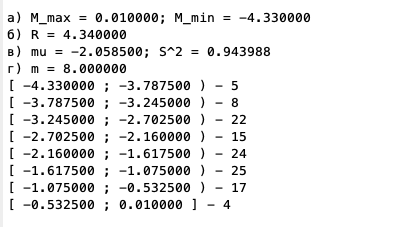
\includegraphics[scale=0.6]{img/res.png}
	\caption{Вывод программы}
	\label{fig:12}
\end{figure}


\begin{figure}[H]
	\centering
	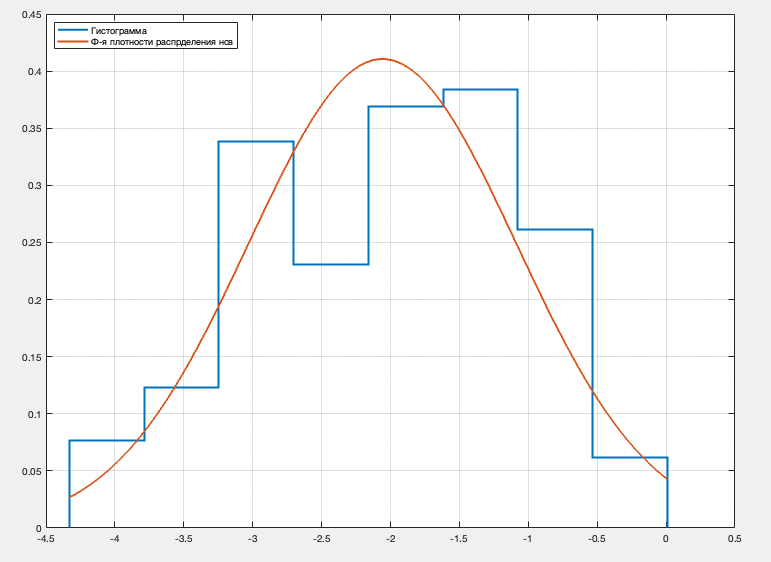
\includegraphics[scale=0.6]{img/1.png}
	\caption{Гистограмма и график функции плотности распределения вероятностей нормальной случайной величины с выборочными мат. ожиданием и дисперсией}
	\label{fig:1}
\end{figure}

\begin{figure}[H]
	\centering
	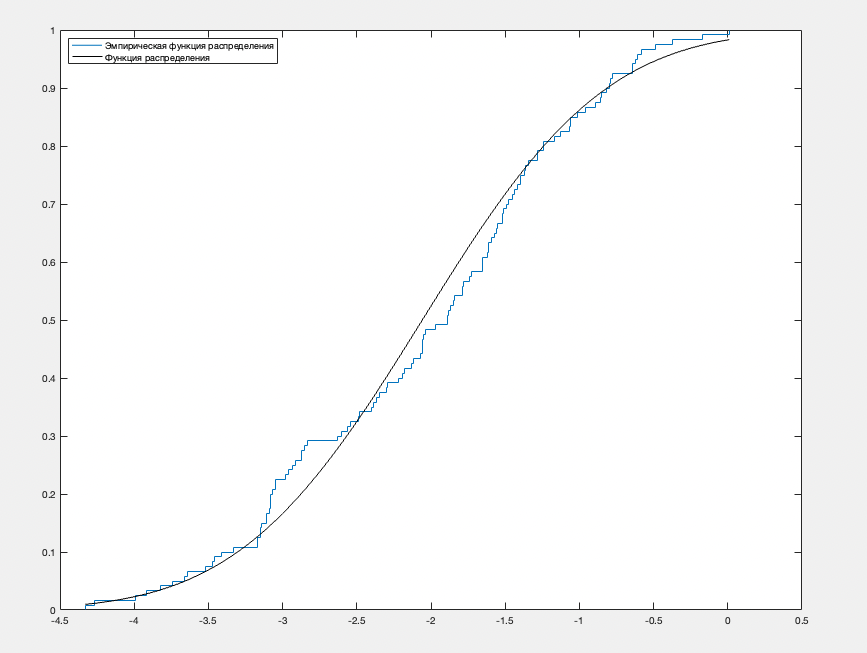
\includegraphics[scale=0.6]{img/2.png}
	\caption{График эмперической функции распределения и функции распределения нормальной случайной величины с выборочными мат. ожиданием и дисперсией}
	\label{fig:2}
\end{figure}

\bibliographystyle{utf8gost705u}  % стилевой файл для оформления по ГОСТу
\bibliography{51-biblio}          % имя библиографической базы (bib-файла)
	
\end{document}
